\section{Alan Turing}

\centerline{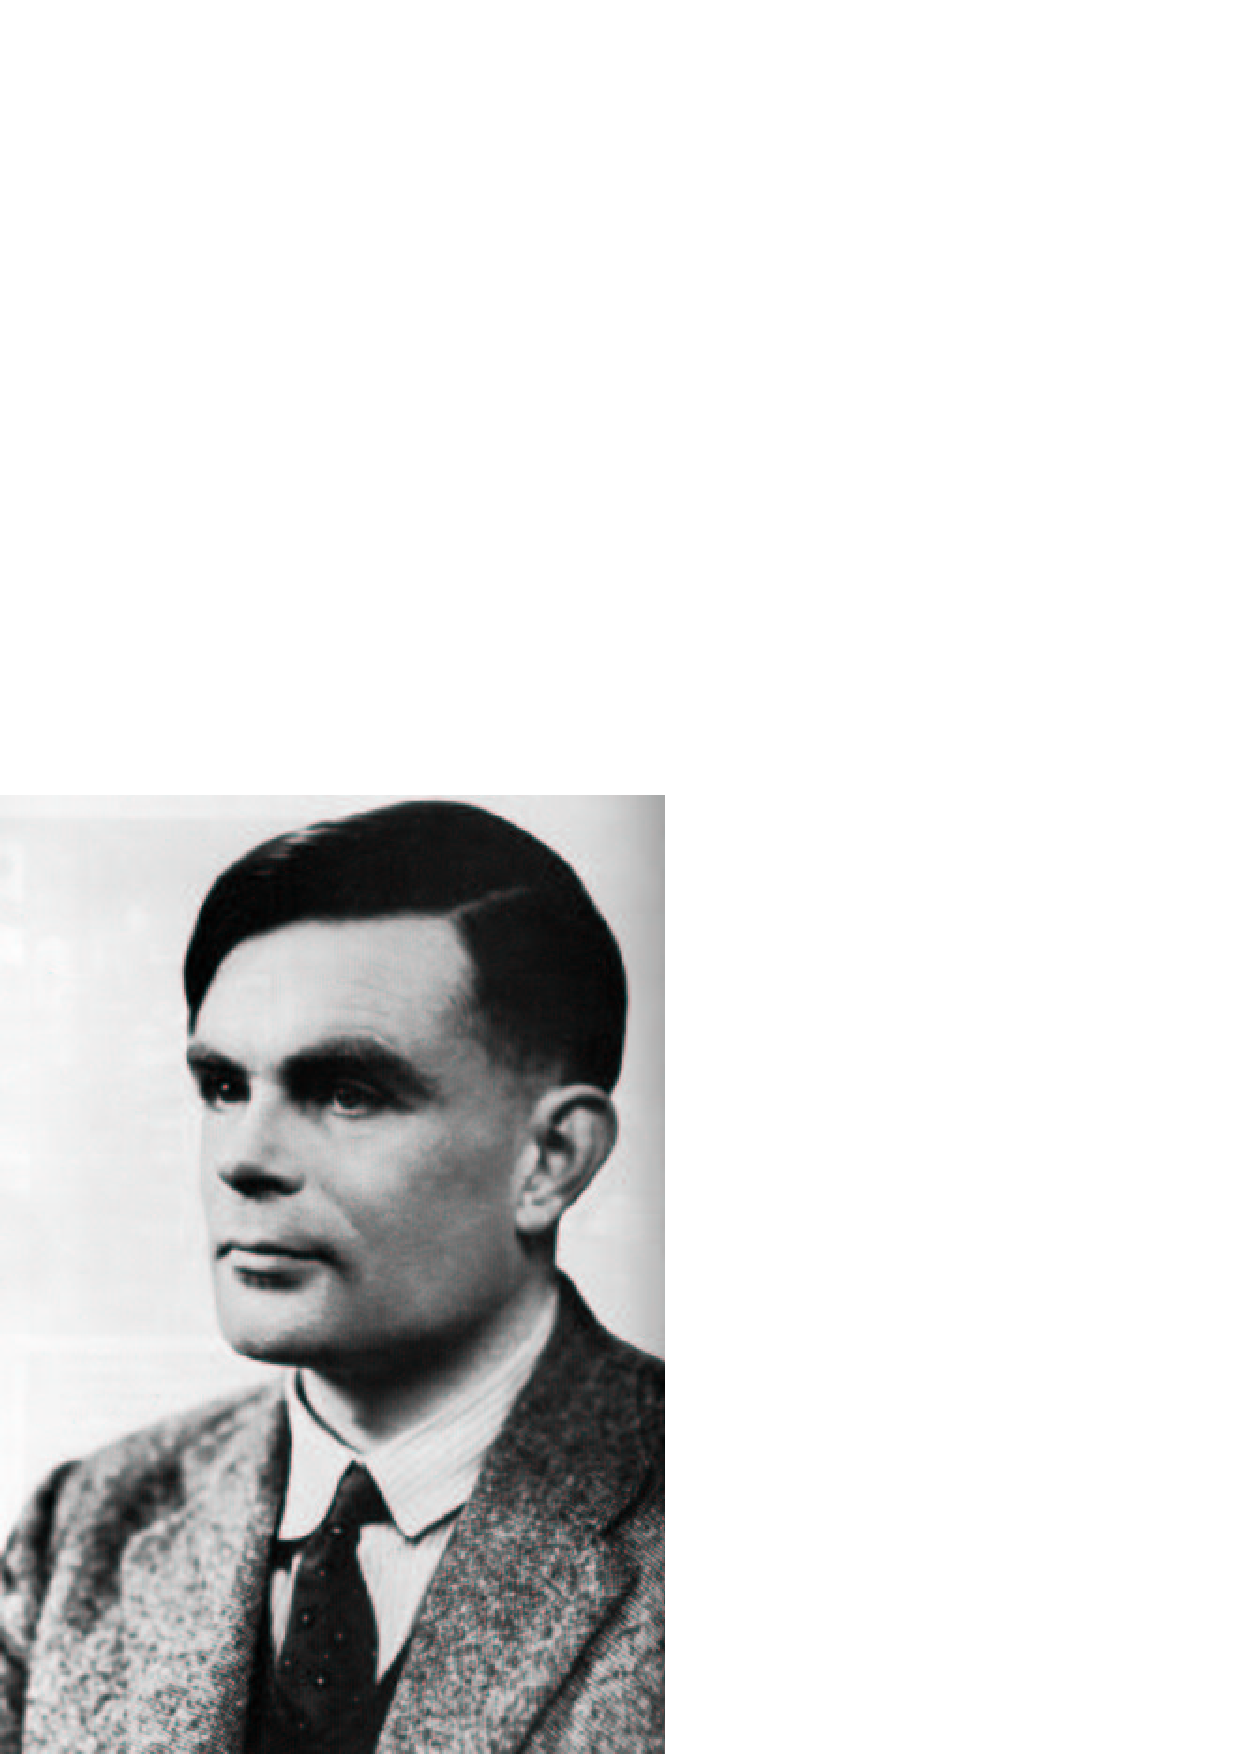
\includegraphics[width=2in]{figures/turing.pdf}}

The man pictured above is Alan Turing, the most important figure in
the history of computer science.  For decades, his fascinating life
story was shrouded by government secrecy, societal taboo, and even his
own deceptions.

At 24 Turing wrote a paper entitled \textit{On Computable Numbers, with an
Application to the Entscheidungsproblem}.  The crux of the paper was an
elegant way to model a computer in mathematical terms.  This was a
breakthrough, because it allowed the tools of mathematics to be brought to
bear on questions of computation.  For example, with his model in hand,
Turing immediately proved that there exist problems that no computer can
solve--- no matter how ingenious the programmer.  Turing's paper is all the
more remarkable because he wrote it in 1936, a full decade before any
electronic computer actually existed.

The word ``Entscheidungsproblem'' in the title refers to one of the 28
mathematical problems posed by David Hilbert in 1900 as challenges to
mathematicians of the 20th century.  Turing knocked that one off in
the same paper.  And perhaps you've heard of the ``Church-Turing
thesis''?  Same paper.  So Turing was obviously a brilliant guy who
generated lots of amazing ideas.  But this lecture is about one of
Turing's less-amazing ideas.  It involved codes.  It involved number
theory.  And it was sort of stupid.

%\subsection{Turing's Code}

Let's look back to the fall of 1937.  Nazi Germany was rearming under
Adolf Hitler, world-shattering war looked imminent, and--- like us--- Alan
Turing was pondering the usefulness of number theory.  He foresaw that
preserving military secrets would be vital in the coming conflict and
proposed a way \textit{to encrypt communications using number theory}.
This is an idea that has ricocheted up to our own time.  Today, number
theory is the basis for numerous public-key cryptosystems, digital
signature schemes, cryptographic hash functions, and digital cash systems.
Every time you buy a book from Amazon, check your grades on WebSIS, or use
a PayPal account, you are relying on number theoretic algorithms.
Furthermore, military funding agencies are among the biggest investors in
cryptographic research.  Sorry Hardy!

Soon after devising his code, Turing disappeared from public view, and
half a century would pass before the world learned the full story of
where he'd gone and what he did there.  We'll come back to Turing's
life in a little while; for now, let's investigate the code Turing
left behind.  The details are uncertain, since he never formally
published the idea, so we'll consider a couple of possibilities.

\subsection{Turing's Code (Version 1.0)}

The first challenge is to translate a text message into an integer so
we can perform mathematical operations on it.  This step is not
intended to make a message harder to read, so the details are not too
important.  Here is one approach: replace each letter of the message
with two digits ($A = 01$, $B = 02$, $C = 03$, etc.) and string all
the digits together to form one huge number.  For example, the message
``victory'' could be translated this way:
%
\begin{center}
\begin{tabular}{ccccccccc}
   &``v &  i &  c &  t & o & r & y'' \\
$\rightarrow$ & 22 & 09 & 03 & 20 & 15 & 18 & 25
\end{tabular}
\end{center}
%
Turing's code requires the message to be a prime number, so we may
need to pad the result with a few more digits to make a prime.  In
this case, appending the digits 13 gives the number 2209032015182513,
which is prime.

Now here is how the encryption process works.  In the description
below, $m$ is the unencoded message (which we want to keep secret),
$m^*$ is the encrypted message (which the Nazis may intercept), and
$k$ is the key.

\begin{description}

\item[Beforehand] The sender and receiver agree on a secret key, which
is a large prime $k$.

\item[Encryption] The sender encrypts the message $m$ by computing:
\[
m^* = m \cdot k
\]

\item[Decryption] The receiver decrypts $m^*$ by computing:
\[
\frac{m^*}{k} = \frac{m \cdot k}{k} = m
\]

\end{description}

For example, suppose that the secret key is the prime number $k =
22801763489$ and the message $m$ is ``victory''.  Then the encrypted
message is:
%
\begin{align*}
m^* & = m \cdot k \\
   & = 2209032015182513 \cdot 22801763489 \\
   & = 50369825549820718594667857
\end{align*}

There are a couple of questions that one might naturally ask about Turing's
code.

\begin{enumerate}

\item How can the sender and receiver ensure that $m$ and $k$ are
prime numbers, as required?

The general problem of determining whether a large number is prime or
composite has been studied for centuries, and reasonably good primality
tests were known even in Turing's time.  In 2002, Manindra Agrawal, Neeraj
Kayal, and Nitin Saxena announced a primality test that is guaranteed to
work on a number $n$ in about $(\log n)^{12}$ steps, that is, a number of
steps bounded by a twelfth degree polynomial in the length (in bits) of
the input, $n$.  This definitively places primality testing way below the
problems of exponential difficulty.  Amazingly, the description of their
breakthrough algorithm was only thirteen lines long!

Of course, a twelfth degree polynomial grows pretty fast, so the
Agrawal,\emph{ et al.}\ procedure is of no practical use.  Still, good
ideas have a way of breeding more good ideas, so there's certainly hope
further improvements will lead to a procedure that is useful in practice.
But the truth is, there's no practical need to improve it, since very
efficient \emph{probabilistic} procedures for prime-testing have been
known since the early 1970's.  These procedures have some probability of
giving a wrong answer, but their probability of being wrong is so tiny
that betting on their answers is the best bet you'll ever make.

\item Is Turing's code secure?

The Nazis see only the encrypted message $m^* = m \cdot k$, so
recovering the original message $m$ requires factoring $m^*$.  Despite
immense efforts, no really efficient factoring algorithm has ever been
found.  It appears to be a fundamentally difficult problem, though a
breakthrough someday is not impossible.  In effect, Turing's code puts
to practical use his discovery that there are limits to the power of
computation.  Thus, provided $m$ and $k$ are sufficiently large, the
Nazis seem to be out of luck!

\end{enumerate}

This all sounds promising, but there is a major flaw in Turing's code.

\subsection{Breaking Turing's Code}

Let's consider what happens when the sender transmits a
\textit{second} message using Turing's code and the same key.  This
gives the Nazis two encrypted messages to look at:
%
\[
m_1^* = m_1 \cdot k
\hspace{0.75in} \text{and} \hspace{0.75in}
m_2^* = m_2 \cdot k
\]
%
The greatest common divisor of the two encrypted messages, $m_1^*$ and
$m_2^*$, is the secret key $k$.  And, as we've seen, the $\gcd$ of two
numbers can be computed very efficiently.  So after the second message is
sent, the Nazis can recover the secret key and read \textit{every}
message!

It is difficult to believe a mathematician as brilliant as Turing
could overlook such a glaring problem.  One possible explanation is
that he had a slightly different system in mind, one based on
\textit{modular} arithmetic.

\endinput